\chapter{User documentation}
\label{ch:user}

In this chapter we will discuss the installation steps,
the correct way of using the software and a brief description
about the software.


\section{Project Description}
\label{s:project_desc}

My project is a desktop application that is meant to run 
on the background while using Mastodon social media. The
whole project was built using the latest \textit{Python} 3 version.
The main goal of the project is to detect possible
threats coming from other accounts in form of direct
messages and tags, after warning the user about possible 
threats it let's the user decide the kind of action
he wants to take against the account that may be a threat
and the domain where the account came from.
\newline
As a prerequisite for using this desktop application is
a stable internet connection and a Mastodon account.


\section{Installation guide}
\label{s:installation_guide}
As earlier mentioned, in order to use Mastodon social media threat alert application
we need to have a stable internet connection and a Mastodon account in any server and Python 3.10.2.
\newline
The application is currently supporting Windows and Linux but the goal is to extend it as a 
mobile application which supports IOS and Android. Hence, the installation steps are the same for
both, Windows and Linux, but we will go through the steps in Windows specifically.
\newline
To download the application we need to clone the following repository: 
\url{https://github.com/DionKajdomcaj/Mastodon-Social-Threat-Alert.git}.
\newline
Prior to cloning the repository we need to make sure that we have git and then use
the following command in the command prompt to clone the repository:
\begin{lstlisting}[caption=Cloning Repository, captionpos=b]
	C:\Users\dionk>git clone https://github.com/DionKajdomcaj/Mastodon-Social-Threat-Alert.git
\end{lstlisting}
After succeeding to clone the repository we need to install the requirements for
our environment. In the repository there is a file called requirements and installing it
will fulfill the requirements to run the application. We can install them by
using the following command in command prompt:
\begin{lstlisting}[caption=Installing requirements, captionpos=b]
	C:\Users\dionk\Mastodon-Social-Threat-Alert>pip install -r requirements.txt
\end{lstlisting}
Now we are ready to run the application.

\subsection{Running the application}
\label{ss:running_app}
In order to run the application we need to make sure that
we are in the correct directory and then run the following command:
\begin{lstlisting}[caption=Running the application, captionpos=b]
	C:\Users\dionk\Mastodon-Social-Threat-Alert>python ThreatAlert.py 
\end{lstlisting}

After running the command, if all the prerequisites are met, we can see 
our application log in page.
\begin{figure}[H]
	\centering
	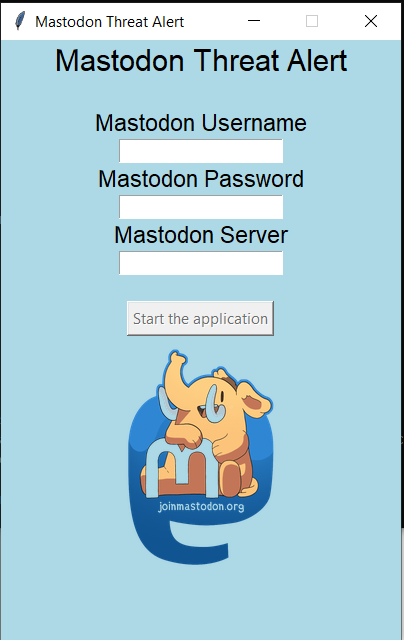
\includegraphics[width=0.3\textwidth,height=240px]{images/mainpageapp.png}
	\caption{Application main page}
	\label{fig:empty_page}
\end{figure}

\section{Logging in}
\label{s:Logging_in}
As we saw in Figure 2.1 the button to actually start the application is disabled.
In order to enable it we must fulfill the requirements which are: filling the username
, password and server field. If only one of them is missing then the user will not be able
to start the application nor use it. 
\begin{figure}[H]
	\centering
	\subcaptionbox{Missing password field - Button disabled}{
		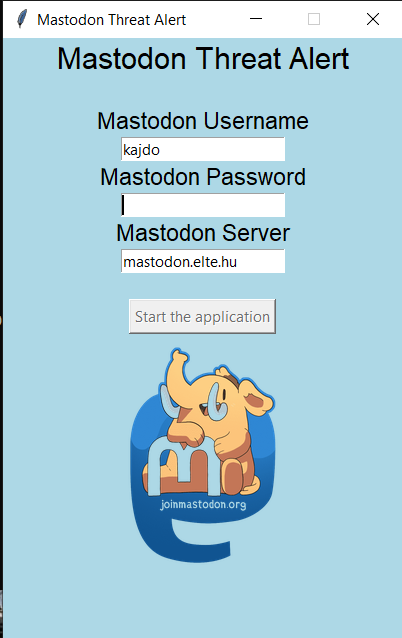
\includegraphics[width=0.45\linewidth, height=240px]{images/buttondisabled.png}}
	\hspace{5pt}
	\subcaptionbox{No missing field - Button enabled}{
		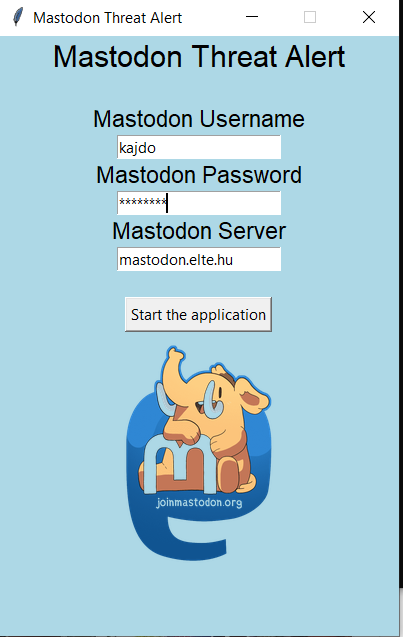
\includegraphics[width=0.45\linewidth, height=240px]{images/buttonenabled.png}}
	\caption{Button disabled and enabled}
	\label{fig:buttonenabled}
\end{figure}
The fields must be filled with the Mastodon account information.
\newline
In the username field you must enter your Mastodon username, and the
same goes up to password. About the server you need to know which server
are you in and only type the domain, for example in case there is an account
like: example@mastodon.social then the username is example and the server is
mastodon.social. All of the data are case sensitive, so you must give them
exactly as they are originally.

\subsection{Correct log in data}
\label{ss:correct_data}
If every data is correct then the application will be connected to the Mastodon API after
we click on the button. The program will let us now that it is running, and it will not
change it's state until it recognizes a possible threat for the logged in user.
\begin{figure}[H]
	\centering
	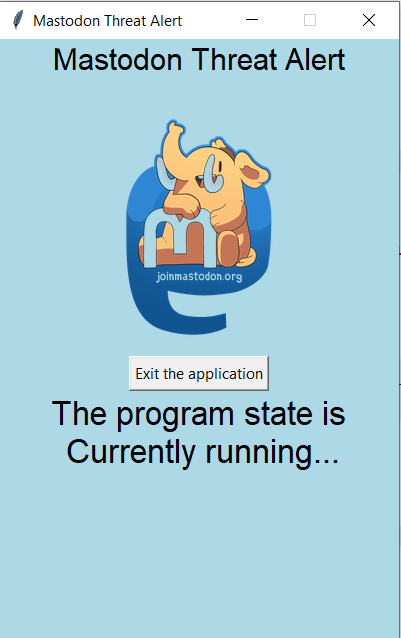
\includegraphics[width=0.3\textwidth,height=240px]{images/runningapp.png}
	\caption{Application running}
	\label{fig:running_app}
\end{figure}

\subsection{Incorrect log in data}
\label{ss:incorrect_data}
Even if the button is enabled it does not mean that the log in data entered by the user
are correct. So, if the user does not give the valid log in data then the application 
will not be connected to Mastodon API. Hence, it will give the user an error message.
The following figure is going to show you the message you will receive for giving invalid 
log in data. After receiving the message you can just press the message button and try again
as many times as you need.
\begin{figure}[H]
	\centering
	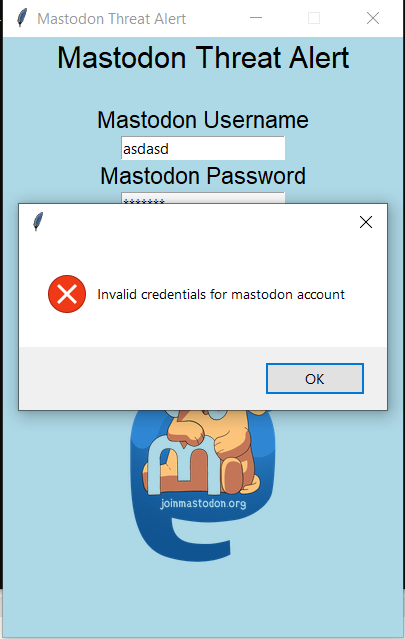
\includegraphics[width=0.3\textwidth,height=240px]{images/invalidred.png}
	\caption{Incorrect log in data}
	\label{fig:invalid_data}
\end{figure}

\section{Actions for the possible threat account}
\label{s:Actions_threat}
Now that we logged in successfully, we can start using Mastodon as usually, but this
time we have the Mastodon threat alert application running on the background and looking
for possible threats.
\newline
Every time that we are going to receive a direct message or a tag notification, that account's
data is going to be checked whether it has a possibility to be a threat or not. After checking
if the account, that was trying to reach you, is considered to be a possible threat, the application
will show you a warning message containing the possible threat account username and domain,
and will ask you to take a certain action against the account.
\begin{figure}[H]
	\centering
	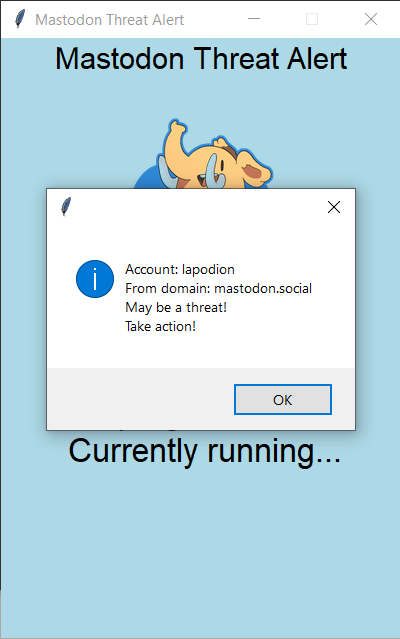
\includegraphics[width=0.3\textwidth,height=240px]{images/threatnotif.png}
	\caption{Possible threat notification}
	\label{fig:possible_threat_notification}
\end{figure}

We have two kind of actions supported in our application which are: Trust and block,
and they are applicable for the possible threat account or the possible threat account's
domain. The default value for both of them is Trust which can be changed.
\newline
We have to simply choose the action from a combo box for both, possible threat account and
it's domain, and click the button in order to perform the actions. 
\begin{figure}[H]
	\centering
	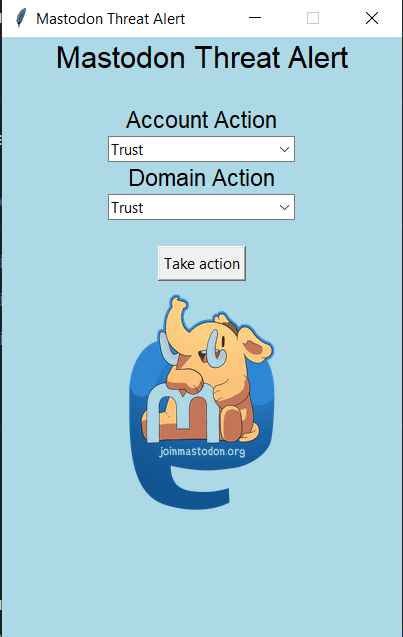
\includegraphics[width=0.3\textwidth,height=240px]{images/actionspage.png}
	\caption{Action window}
	\label{fig:action_page}
\end{figure}
Now we can choose independently the type of action for both, the account
and it's domain.
\newline
After clicking the button the actions will take place
and the application will go to it's running state again.
\begin{figure}[H]
	\centering
 	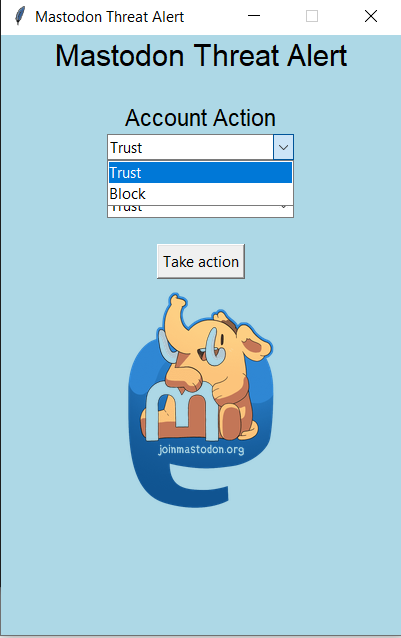
\includegraphics[width=0.3\textwidth,height=240px]{images/actiontypes.png}
	\caption{Choosing the type of action}
	\label{fig:choosing_action}
\end{figure}

\subsection{Account action}
\label{ss:acc_action}
As it was mentioned before that we can choose the actions separately for the possible threat account and it's
domain. In both cases we have Trust and Block as actions, but they behave differently
as account action and as domain action.
\newline
In case of the account the Trust action just trusts the account and does not check it
again if it tries to reach you. However, the Block action blocks the account completely,
and that account will not be able to reach you in any form.
\subsection{Domain action}
\label{ss:dmn_action}
In case of the account's domain the trust action works the same as in the account action.
However, in case of the Block action the domain is going to be blocked and the user will not
receive any notifications from accounts that have the blocked domain.



